\justifying
\NSFCBodyText

\subsubsection{研究内容}
本项目围绕长程任务中的“状态保留—证据恢复—预算调度”研究三个相互依赖的环节。研究内容一识别当前任务尚需保留的约束和证据关系，研究内容二以这些关系指导卸载与有效恢复，研究内容三根据恢复风险和资源余量选择操作，并通过共同实验检验各环节的独立与联合贡献。核心对象为文本和工具调用轨迹，不开展基座大模型预训练；多模态信息只在工具已经形成可追溯文本结果时接入。

\textbf{研究内容一：任务状态感知的保真压缩。}将轨迹划分为用户要求、未完成子目标、已执行动作、工具观察与证据引用，研究这些信息的后续任务价值。重点不是让摘要尽可能详细，而是识别会改变动作合法性、对象选择或子目标衔接的信息。拟比较基于近因、文本显著性和动作依赖的保留策略，研究有限摘要长度下哪些状态应原样保留，哪些内容可转为结构化事实，哪些内容可只保存原文索引。输出为带来源关联的紧凑任务状态和信息价值估计，供第二项研究确定卸载方式，并向第三项提供压缩失真风险。

\textbf{研究内容二：动作依赖引导的证据卸载与有效恢复。}在保留不可变原始记录的前提下，将长工具结果移出工作上下文，研究如何依据待执行动作的前置条件选择回取对象。恢复时联合检查对象标识、来源版本及适用条件；对可能过期的证据向环境重查，并记录校验失败。重点分析依赖保留与版本检查的交互效应，区分因摘要遗漏、索引遗漏、版本过期及执行误用造成的错误。输出为经核对的证据片段、仍未满足的前提及实际回取开销，为调度提供反馈。

\textbf{研究内容三：计及全开销的自适应调度与可靠性验证。}以固定执行模型为基础，研究在保留、压缩、卸载、恢复及重查之间选择操作的规则与轻量策略。调度依据包括上下文占用、未完成依赖、候选证据风险和剩余资源；硬约束始终由实际计数执行。通过公开交互环境及受控扰动，检验整个系统在任务长度、噪声与版本变化条件下的成本—成功率关系，确定能实现净收益的区间及失效原因。

\subsubsection{研究目标}
总体目标是在固定执行模型和共同资源边界下，形成可追溯的上下文管理方法，明确压缩、有效恢复与长程任务可靠性的关系。项目拟实现三个可检验子目标：识别能稳定降低动作前提丢失的状态保留方式；验证动作依赖与有效性校验是否对过期证据引起的失败产生可重复影响；给出包含全部控制开销的成本—成功率比较及适用范围。

核心验收以公开环境的程序化任务终态为准，同时报告约束违例、有效证据恢复、峰值上下文和端到端时延。\textbf{【暂定 核心工作点以任务成功率相对强基线下降不超过3个百分点为非劣界，争取累计Token减少30\%】}。这些数值是待先导实验校准的设计目标，既不是已有结果，也不替代官方合同指标。若该工作点不能达到，仍须报告完整权衡关系、失败分型及可复现对照，而不能只选择最有利的压缩率。

\subsubsection{拟解决的关键科学问题}
\textbf{哪些信息在压缩后仍应作为任务状态保留？}同一句约束的价值可能随目标完成和环境变化而改变。拟研究以未完成动作的前置条件和证据关系表征未来需要，能否比文本显著性或最近访问时间更有效地保护关键状态，并分析这种优势对依赖跨度及观测不确定性的敏感性。

\textbf{原文回取何时构成对当前动作有效的证据恢复？}拟把恢复分解为定位、读取与适用性核对。通过独立操纵依赖保留和版本校验，分析二者是否存在可复核的交互作用。重点研究依赖记录被压缩或元数据不完备而当前状态仍可查询的情境；当前状态既不可见又不可查询时单列为不可充分识别条件。如果正确版本的证据仍不足以改善终态，需继续区分执行模型误用、前提定义错误或任务本身不可完成等原因。

\textbf{可靠性改善何时能够抵消上下文管理开销？}拟分析长工具输出、依赖跨度与更新频率如何改变压缩和回取的价值。研究目标包含无收益和负收益条件；短任务若直接保留历史更合适，调度器应能够选择低干预操作，而非为了展示模块能力而反复压缩。

\subsubsection{研究方法}
\textbf{统一状态与操作定义。}以第\(t\)步前可见历史\(H_t\)、紧凑状态\(Z_t\)、原文档案\(M_t\)与剩余预算\(b_t\)描述研究系统。\(Z_t\)包含当前目标、未完成约束、已执行动作及其证据关联；它是从观察估计的工作状态，不等于环境的完整真实状态。上下文操作记为\(u_t\)，任务动作记为\(a_t\)，二者分开记录，避免把额外控制调用藏入主模型的行动统计。

对候选片段\(e\)，拟估计其省略后导致关键动作错误的条件风险，并结合回取成本形成保留优先级。训练阶段可在可复位环境中比较保留或删除该片段后的执行分支；线上仅使用截至当前步已观察到的目标、动作、工具返回与历史记录。未来轨迹和答案只能用于训练标签与离线诊断，不能作为在线信息价值的输入。若干预分支出现合法替代动作，以前置条件与任务终态判断后果，不以动作字符串一致作为保真标准。

将任务约束失真记为\(D_c\)，未完成子目标丢失记为\(D_g\)，动作—证据依赖遗漏记为\(D_e\)，综合失真\(D_t=w_cD_c+w_gD_g+w_eD_e\)仅作训练与诊断量。权重在开发集设定，其数值不能保证实际任务安全。主要结果仍是环境判定的任务成功率及违例率，通过删除状态项、打乱关联和替换版本的消融检验各项是否具有预测与干预价值。

\textbf{同条件实验体系。}主实验采用 AppWorld 中可复位且具有程序化终态判定的任务\cite{appworld}，跨环境验证采用 WebArena 中具备相应操作接口的任务\cite{webarena}。LongMemEval 的知识更新与时间推理任务作为恢复模块诊断\cite{longmemeval}；LongBench 和 RULER 用于压缩器的静态信息保留检查\cite{longbench,ruler}。SWE-bench 的代码任务只作为条件允许时的扩展，不与主实验争夺同等规模资源。任务清单与排除条件在比较前固定，不按某一方法是否成功来筛选样本。

同一任务集合设置未压缩历史、滑动窗口和固定周期摘要等基础参照。压缩方法采用 LLMLingua-2，外部记忆参照采用 MemGPT 与 ReadAgent 型方法，轨迹管理参照采用 ACON 和 AgentFold 型方法；在代码与资源允许时加入 AgeMem、ContextBudget、MemStrata、PLACEMEM 的相应实现。不同方法按公开代码版本冻结。对不可在同一执行模型上运行的训练型方法，另设原生配置参照，清楚区分“同骨干机制比较”和“原生系统比较”；简化复现不冒充作者实现，也不从跨模型分数直接推导机制优劣。

主干计划采用\textbf{【暂定 两个可本地运行的指令模型档位、三个上下文预算和至少三次重复】}。先以\textbf{【暂定 60个开发任务】}估计任务分歧率、运行成本与扰动可行性，再根据成对分歧率、非劣界与目标功效确定主评测任务数。若样本量不足，明确保留探索性判断，不事后放宽非劣标准。先导阶段同时形成可用独立任务数与所需样本量的对照表，以每种方法单任务实测GPU时、接口调用数和失败重跑率估算总运行量；总量按任务数、比较方法数、种子数和实际保留的扰动层数相乘，再与可分配机时及经费核对。只有独立任务数量与资源两项同时满足时，才启动确认性比较；不足时保持原非劣界，先完成一个环境、一个模型和一个窗口的机制实验，其余配置依次延后，结论限于探索性证据。增加种子不补足独立任务，不能合并开发任务进入测试集。确认性主要比较预先固定为一个主模型、一个窗口工作点与有限元数据强组合基线，其余模型和预算用于迁移及敏感性分析。主测试使用官方可用测试划分，参数、提示词和阈值不在测试结果上调整；同一模板的改写任务、共享环境实例及派生扰动归入同一划分，防止近重复泄漏。外部模型若使用，需记录模型版本、调用日期和采样设置。

\textbf{主要终点与统计分析。}对每个预注册任务记录终态成功、约束违例及成本；超时、拒答、预算耗尽和恢复循环导致的中止都计为任务失败，并在失败原因中单列。不能以更频繁拒答降低违例率后声称成功率提升。统计以任务为单位，多个随机种子、步骤和扰动版本在任务内聚类。主要比较使用成对任务的成功差及任务级自助法置信区间，非劣判断采用预先指定的单侧区间；区间跨越非劣界时结论为证据不足。预先按“任务成功率达到非劣标准、再检验总成本降低”的顺序判断，不在看到测试结果后改选优效或降本终点。多基线和多预算作为次要分析，使用明确的多重比较校正并保留效应量。依赖保留与有效性检查的交互在成功率加性尺度上定义为\(I=p_{11}-p_{10}-p_{01}+p_{00}\)，其中下标表示两个因素是否启用；联合优于单项不能直接证明互补，须将\(I\)与开发阶段确定并预注册的最小有意义幅度比较。

全部方法遵守相同上下文窗口、最大任务动作数、外部接口调用总上限和累计Token预算；原文存储上限与访问接口保持一致。累计Token包括执行、压缩、索引中需要模型的部分、检索改写、有效性校验和失败重试的输入与输出，另列峰值窗口、检索次数、存储量、端到端时延中位数与高分位数。外部接口总调用数同时计入任务操作、控制器重查、恢复触发查询及失败重试，本地档案读取单列；不能仅限制主智能体动作而让控制器额外查询不受限。\textbf{【暂定 外部接口调用上限按开发任务长度分层确定并冻结，各方法采用相同上限】}。推荐工作点还需将外部交互比率的单侧置信区间与开发阶段预注册的容忍界比较；若交互或时延增加，只报告Token与其它代价的权衡，不宣称总体效率提高。离线训练与索引构建开销单列，并报告是否以及按多少任务摊销。价格、缓存和批处理条件与Token物理计数分开，避免不同计费策略造成虚假节省。

\subsubsection{技术路线}
\textbf{总体技术路线。}研究从可复位工具环境的完整轨迹出发，先建立任务状态与原始证据的关联，再比较不同压缩表示对动作前提的保留；长结果写入原文档案后，以未完成动作的证据需要驱动恢复，并通过来源版本与当前环境查询核对适用性；调度器接收压缩风险、恢复结果及预算反馈，选择下一步上下文操作。最终以任务终态、失败分型和全开销核算检验三项研究内容是否共同改善长程执行。
% NSFC-ILLUSTRATED BEGIN F02
如图~\ref{fig:framework} 所示，ACORE以状态保留、有效恢复和预算调度组织上下文管理。
\begin{figure}[htbp]
\centering
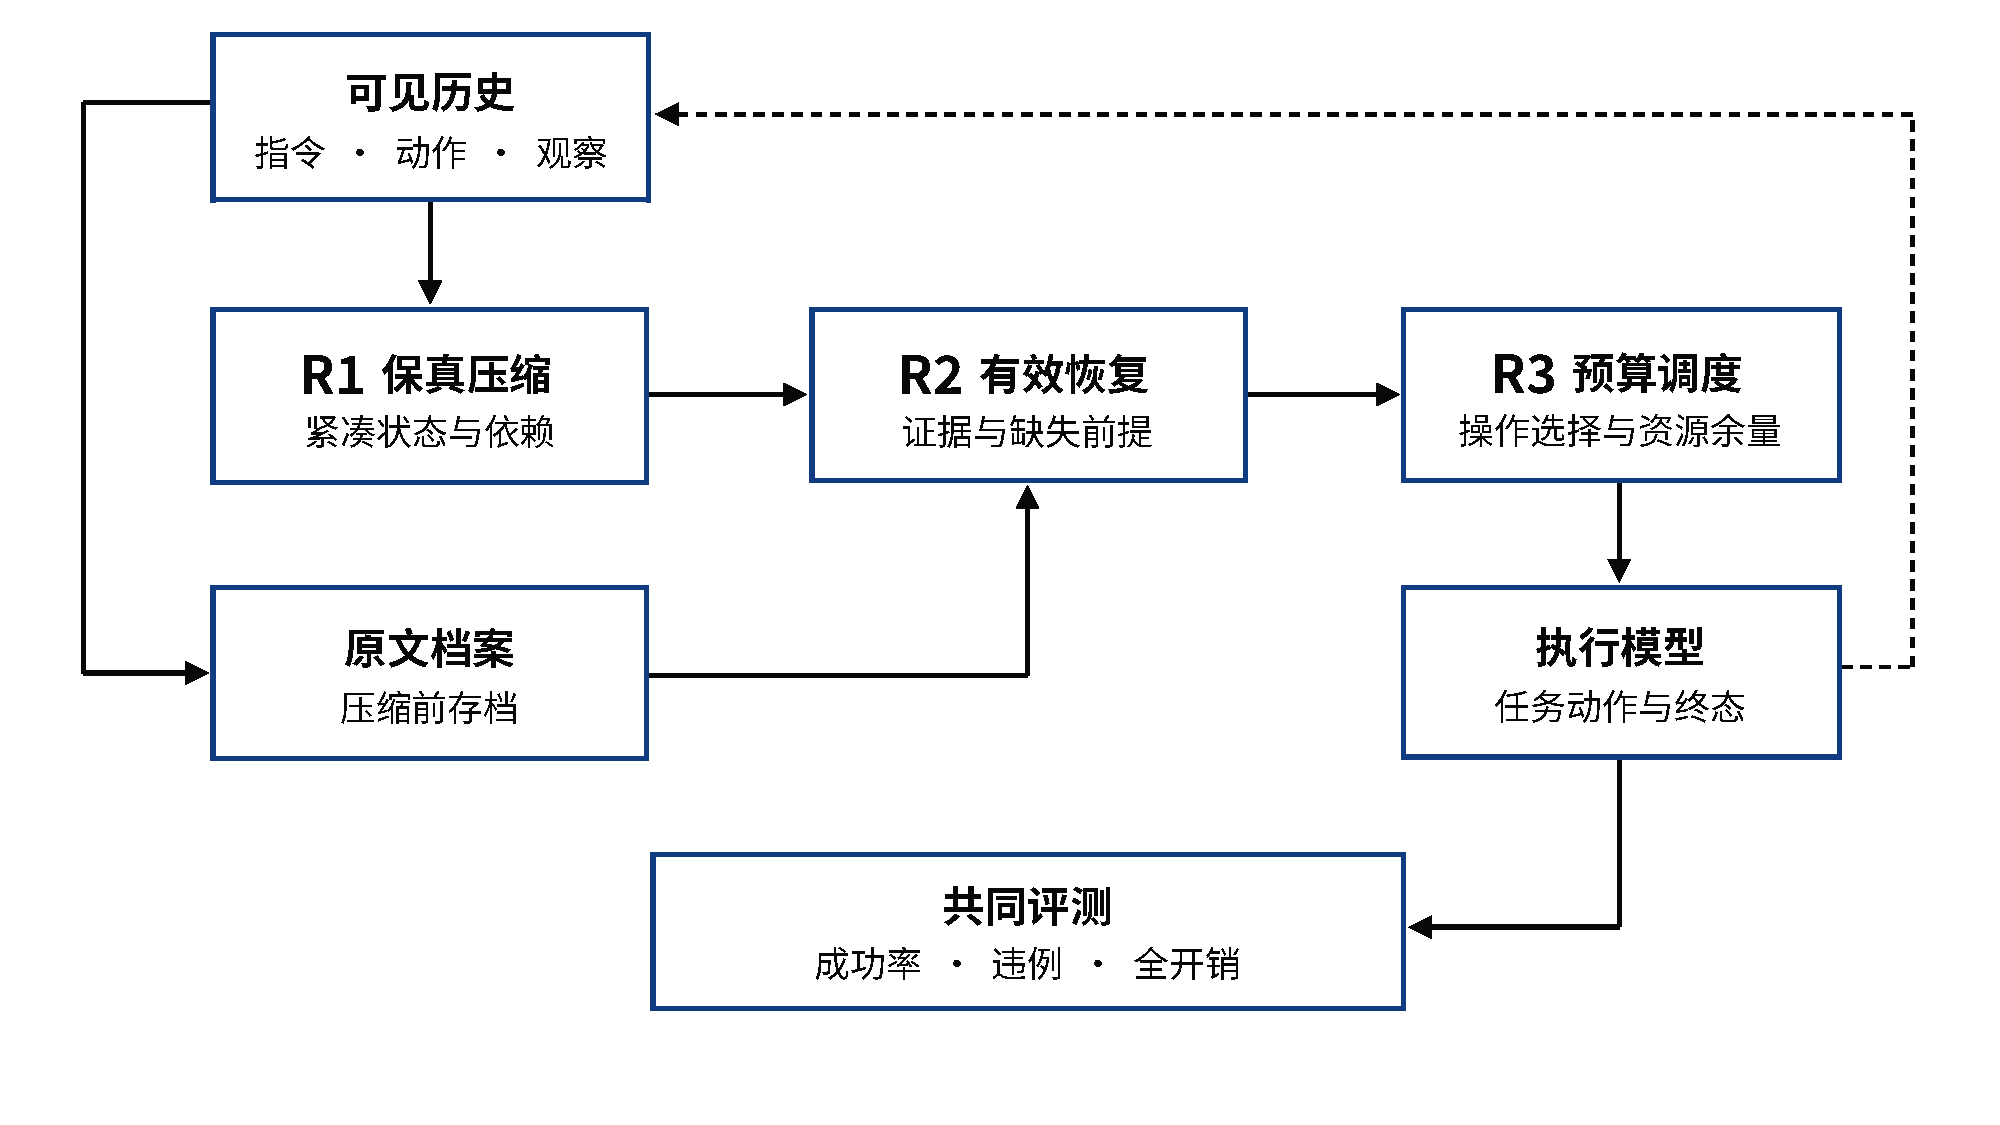
\includegraphics[width=0.98\linewidth]{figures/F02-framework.pdf}
\caption{ACORE以状态保留、有效恢复和预算调度组织上下文管理}
\label{fig:framework}
\end{figure}
% NSFC-ILLUSTRATED END F02


\textbf{面向研究内容一的任务状态保真压缩路线。}输入为当前指令、已执行动作、工具观察和已知未完成目标。首先提取对象、约束、动作前提及证据关联，区别已完成目标与仍需履行的要求；随后在相同长度预算下形成原文片段保留、结构化事实和子任务概要三种粒度的表示。禁止修改用户约束的逻辑方向、对象标识及仍有效的数值条件。对来源未明或提取不确定的关键内容优先保留原文，并把不确定性作为风险特征。

信息价值模型优先采用可解释特征与轻量分类器，以当前目标相关性、依赖是否未完成、信息是否被更新以及回取难度估计保留需求。通过可复位环境中的片段删除和恢复分支获得训练信号，不把全历史成功轨迹一律作为正确标签。样本中同时包含可解、失败和存在多个合法动作的任务，对标注分歧建立人工复核子集。若轻量模型未稳定优于规则基线，保留规则方案完成后续机制研究。

这一分路线输出紧凑状态、关联证据索引和保真风险。验证比较相同摘要长度下的关键约束遗漏率、动作前提满足情况与任务终态，并以去掉依赖关系、去掉未完成目标、随机保留等消融排除单纯长度优势。其输出直接作为下一分路线的恢复请求依据；不能由恢复模块看到压缩模块未被允许使用的未来答案。
% NSFC-ILLUSTRATED BEGIN F03
如图~\ref{fig:compression} 所示，R1依据未完成动作依赖选择压缩表示并保留来源索引。
\begin{figure}[htbp]
\centering
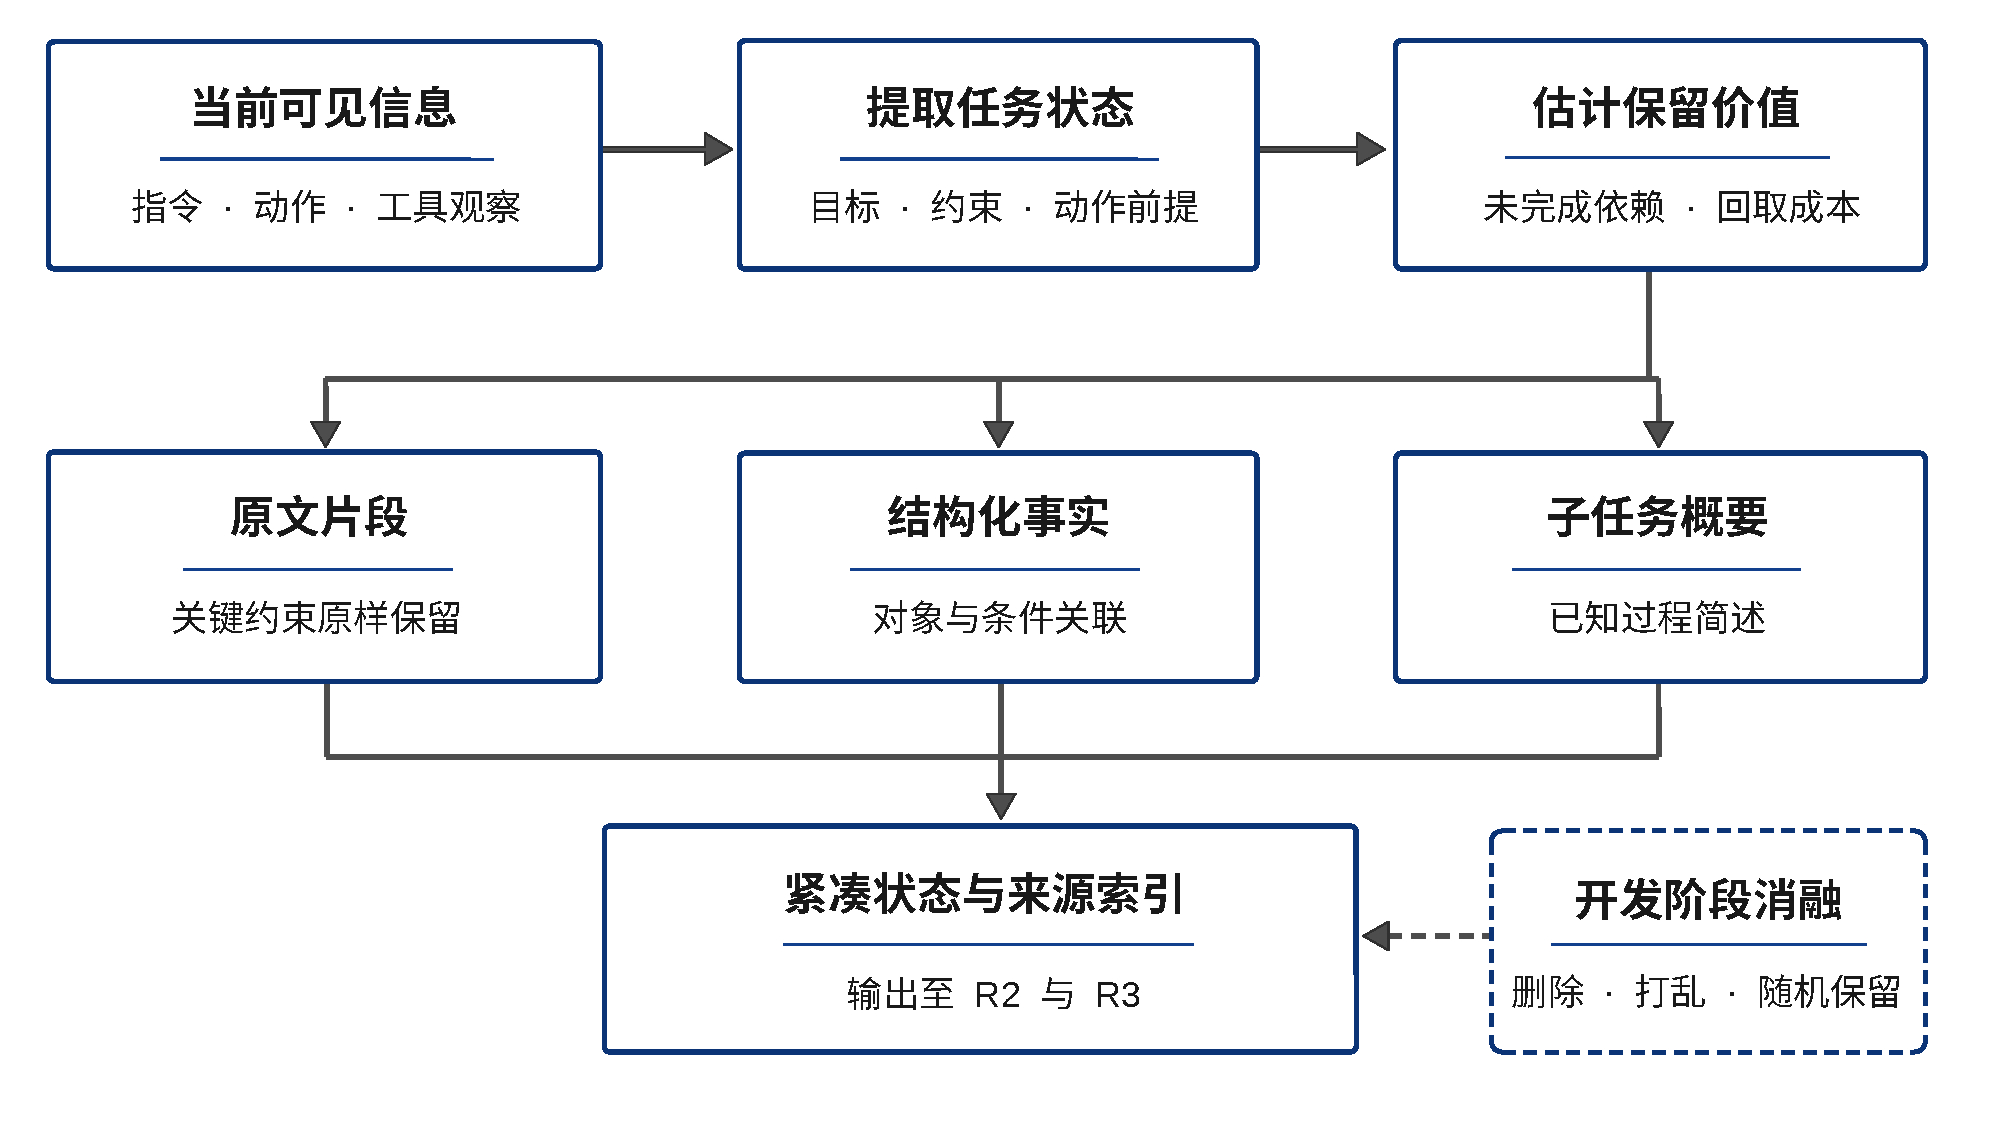
\includegraphics[width=0.98\linewidth]{figures/F03-compression.pdf}
\caption{R1依据未完成动作依赖选择压缩表示并保留来源索引}
\label{fig:compression}
\end{figure}
% NSFC-ILLUSTRATED END F03


\textbf{面向研究内容二的证据卸载与有效恢复路线。}输入为紧凑状态、拟执行动作及其缺失前提。每份工具结果在压缩前存入不可变档案，并建立来源、对象、版本、时间和访问条件的关联；卸载只移出工作窗口，不删除档案。概要记录指向具体原始片段，后续更新创建新版本并保留版本关系。在环境不提供版本号时，使用读取时间、来源快照及必要重查描述新旧关系，不把自定义哈希视作业务版本。

恢复先由动作前提生成候选请求，再结合对象过滤、语义匹配与来源关联选取片段。读取后分两层核对：哈希检查字节完整性，对象及有效期检查描述是否适用于当前动作；可能被外部操作改变的关键状态通过环境接口重新查询。对无法确定的前提，优先请求更完整原文或重查；资源不足时结束该次任务并记录失败，不能凭近似摘要继续执行需确定证据的操作。恢复到旧原文属于可追溯回读，不等于摘要可逆或环境回滚。

核心机制实验采用“保留动作依赖/不保留动作依赖”与“核验当前有效性/不核验当前有效性”的交叉设计。四组共享原文档案、执行模型和候选证据规模，并在局部机制回放中匹配Token与实际查询开销，以分离更多上下文带来的影响；完整系统实验只匹配总预算上限，保留自然执行的实际调用差异，不添加无效调用强行配平成本。
% NSFC-ILLUSTRATED BEGIN F06
如图~\ref{fig:experiment} 所示，四组交叉比较在共同条件下检验依赖保留与有效性核验的作用。
\begin{figure}[htbp]
\centering
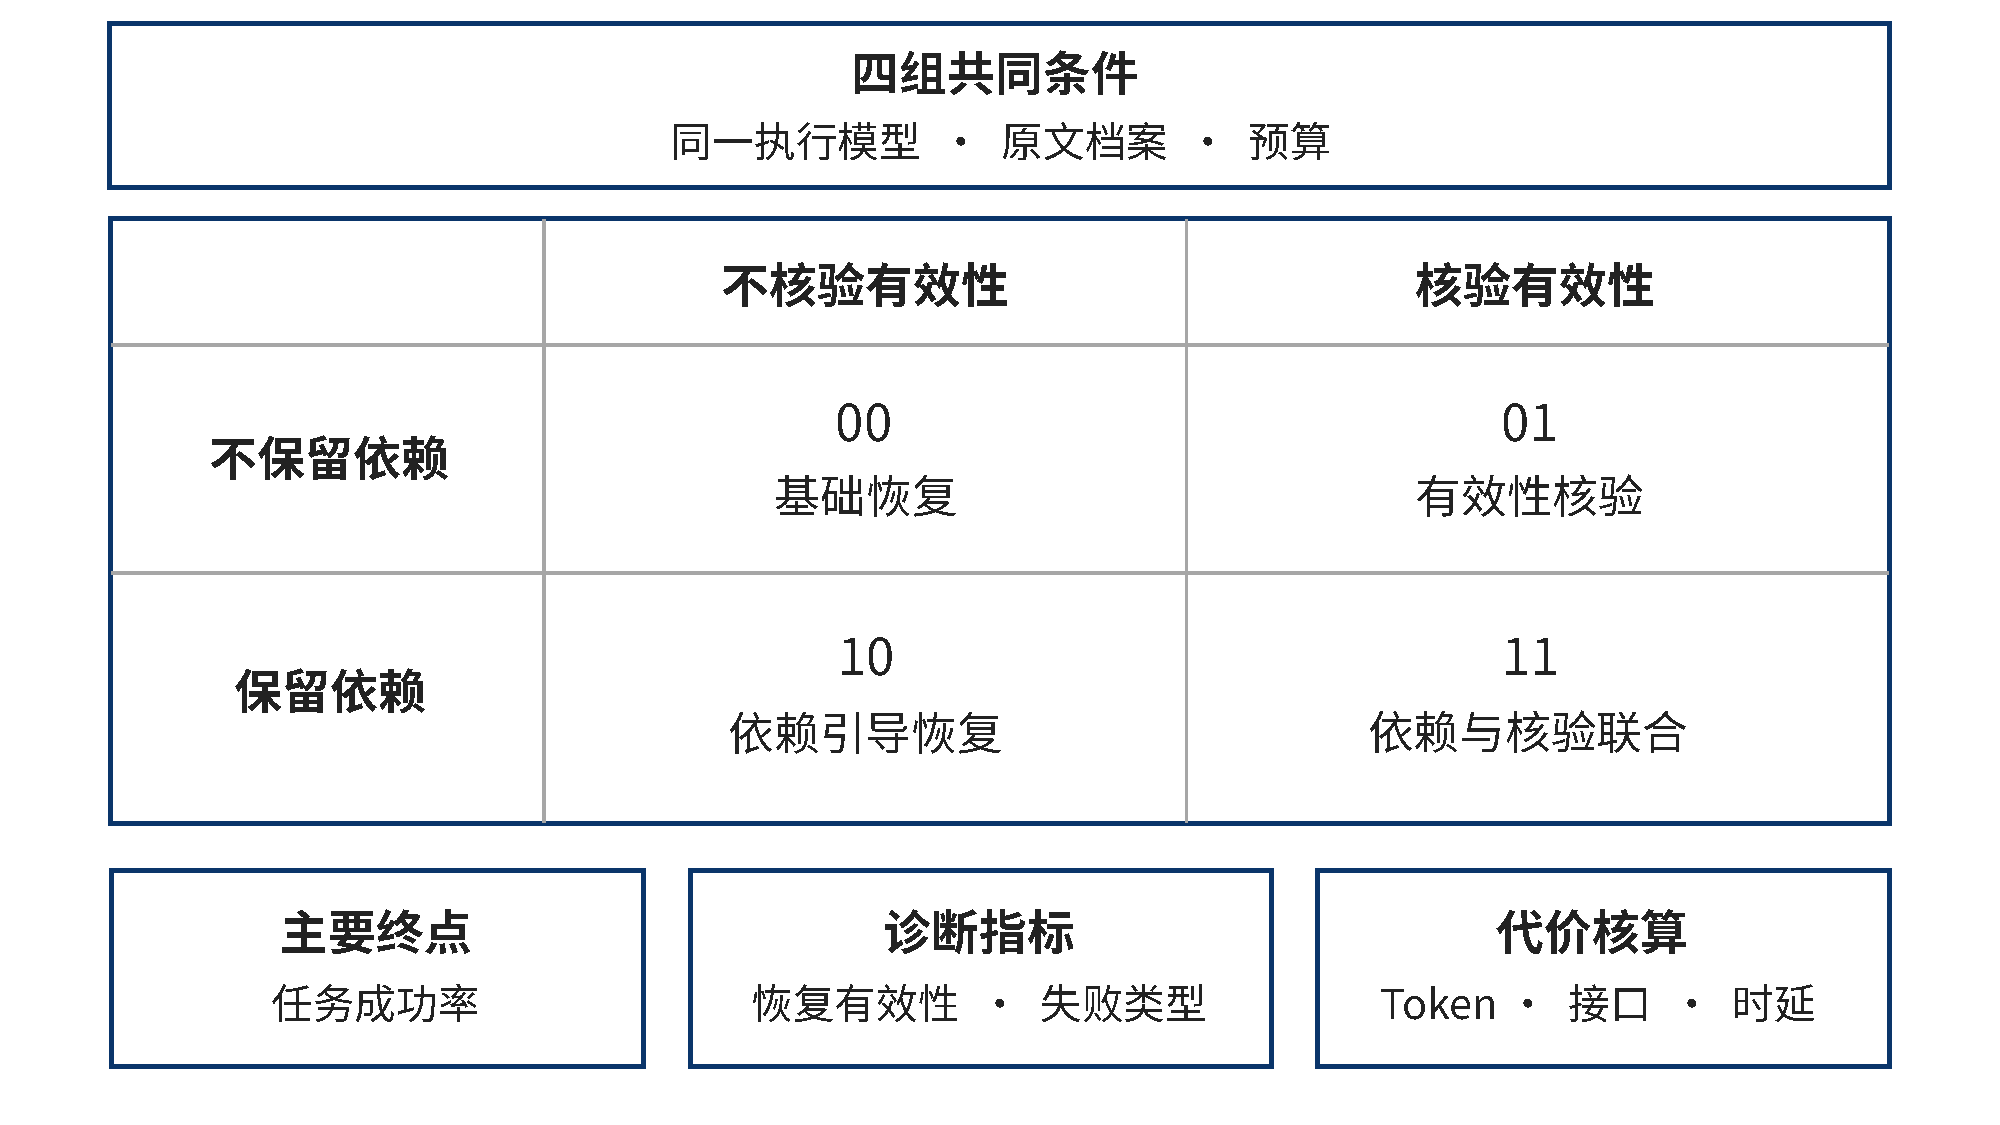
\includegraphics[width=0.98\linewidth]{figures/F06-experiment.pdf}
\caption{四组交叉比较在共同条件下检验依赖保留与有效性核验的作用}
\label{fig:experiment}
\end{figure}
% NSFC-ILLUSTRATED END F06


将“环境原本不提供元数据”与“原本可见、随后被压缩删除”分别干预，线上策略只可使用已识别的前提缺口，不能使用实验者的隐藏缺漏率或未来变更。在此基础上分层改变压缩强度、依赖可见程度与元数据错漏比例，检验有限预算在保留关系和主动取证之间的配置。所有方法获得同等真实元数据，以“有限元数据下的依赖记录、版本过滤与规则重查强组合”为主要对照，并给予相同的调参预算及预算自适应重查能力；比较分配策略时向强基线提供同一可部署缺口识别结果并计费，另做识别器消融，以分离额外信息与分配决策的作用；全量无损元数据加确定性失效仅作诊断参照，每次重查作为高成本参照。

无变更任务和弱依赖任务作为负对照；元数据错漏、索引延迟和无可用新版本作为压力测试。预期若二者配合有效，其影响应集中在跨阶段依赖强、版本变化明显的任务；若单独版本过滤或简单规则组合已达到同等终态表现，则收缩交互机制解释。

此分路线输出经核对的证据、未满足前提与恢复成本。分别记录候选召回、读取完整、当前有效、正确使用四个环节；有效证据恢复率的分母是经独立标注确需回取且原文可用的事件，同时报告所有恢复请求中的失败比例。事件级指标只用于诊断，任务级终态承担主要结论。恢复风险和成本随后反馈给调度器，改变下一轮保留优先级。
% NSFC-ILLUSTRATED BEGIN F04
如图~\ref{fig:recovery} 所示，R2从动作前提出发回读原文并核对证据的当前适用性。
\begin{figure}[htbp]
\centering
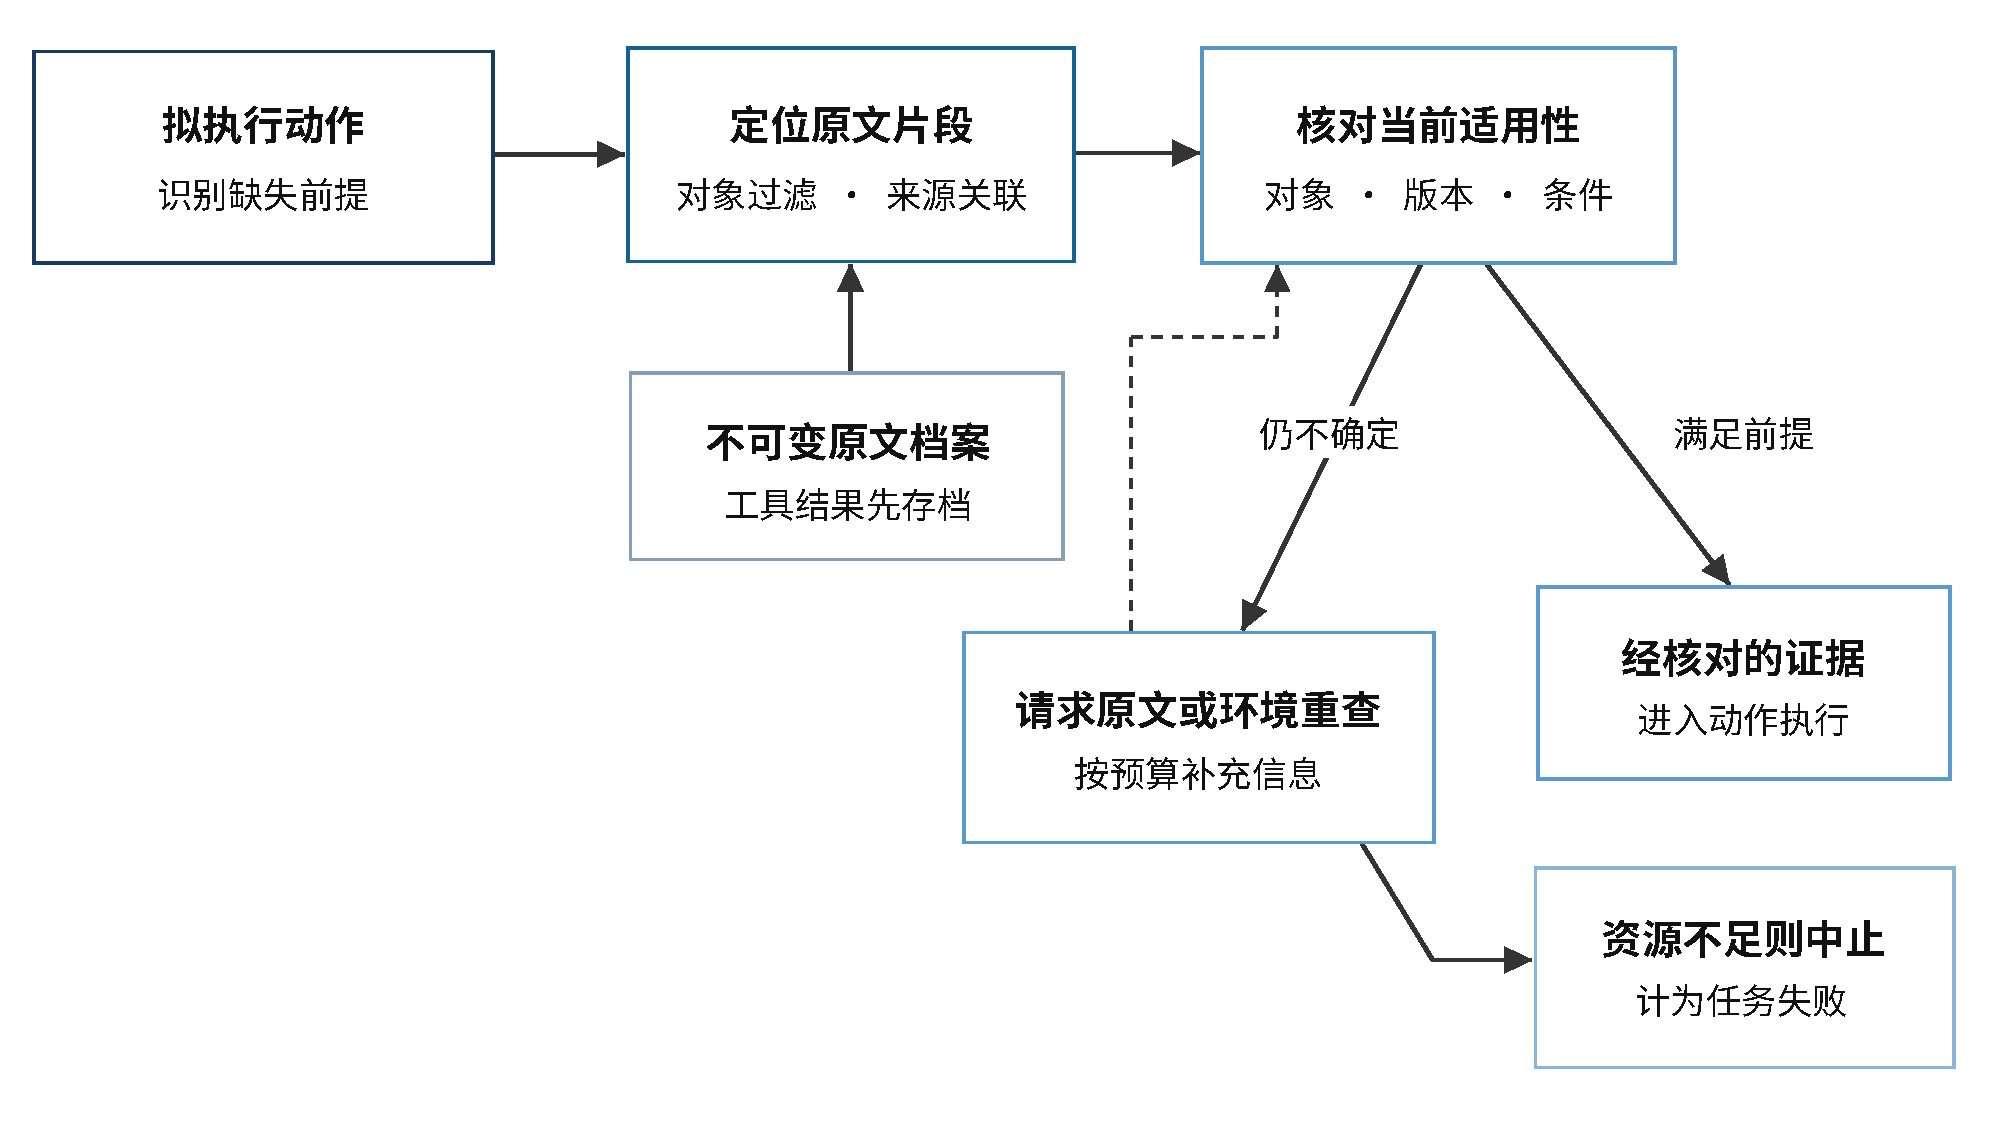
\includegraphics[width=0.98\linewidth]{figures/F04-recovery.pdf}
\caption{R2从动作前提出发回读原文并核对证据的当前适用性}
\label{fig:recovery}
\end{figure}
% NSFC-ILLUSTRATED END F04


\textbf{面向研究内容三的全开销调度与验证路线。}输入为工作状态、原文档案索引、恢复反馈与剩余预算。先建立窗口阈值、固定周期及依赖触发三类规则基线，再使用开发轨迹训练轻量控制器，比较其是否值得额外复杂度。控制器在保留、压缩、卸载、恢复与重查中选择操作；安全性和资源限制通过显式计数及动作前提检查实现，不能交由学习目标隐式保证。

具体而言，在两条候选证据均被同一识别器标为“状态不确定”、且只剩一次重查预算时，强规则按预先调好的风险阈值与近因次序选择；拟研究的策略进一步使用可见的未完成动作依赖、原文重读长度和该对象历次变更记录，估计重查对下一动作前提的边际作用。它可能保留一条较旧但关联关键未完成约束的原文索引，把查询用于即将被修改的对象。该差异属于待检验的决策假设；上述特征也提供给特征规则基线，若规则取得相同效果，就不把学习控制器作为必要创新。

拟研究的约束形式为：
\[
\min_{\pi}\;\mathbb{E}_{\pi}[C_{\mathrm{all}}]\quad
\text{s.t.}\quad
p_{\pi}\ge p_{\mathrm{ref}}-\delta,\qquad
L_t\le B,\qquad C_{\mathrm{all}}\le C_{\max}.
\]
其中\(C_{\mathrm{all}}\)表示单任务全部模型调用Token或同口径资源成本，\(p_{\pi}\)为任务分布上的成功概率，\(p_{\mathrm{ref}}\)为指定强基线成功概率，\(\delta\)为预注册非劣界；\(L_t\)为单次上下文占用，\(B\)和\(C_{\max}\)分别为窗口及累计预算上限。成功概率约束通过独立测试估计，不能在执行前保证；窗口和累计预算由运行器实际强制。若关键约束本身已超窗口，按不可容纳任务记录并计入总体结果，不从总体中静默剔除。

调度训练以已发生的状态和成本为输入，开发阶段可利用完整轨迹形成诊断参照。若采用未来信息决定最优操作，只能将其作为不可部署的理想参照，不能列入线上方案。控制器增加最小操作间隔和恢复次数限制，防止同一证据在压缩与恢复之间循环；阈值在开发集设定，全部额外调用进入核算。最终在不同任务长度、证据依赖跨度、无关输出比例和环境更新频率下比较方法，报告成本—成功率权衡及无收益区间。

三条路线形成可观察的反馈关系：状态表示决定可提出哪些恢复请求，恢复结果暴露表示遗漏及证据过期风险，调度依据这些反馈重新分配有限上下文。共同实验保持这一反馈链可追踪，既做分模块干预，也检查整条轨迹的最终操作结果。
% NSFC-ILLUSTRATED BEGIN F05
如图~\ref{fig:control} 所示，R3结合恢复反馈选择上下文操作并记录全部调用成本。
\begin{figure}[htbp]
\centering
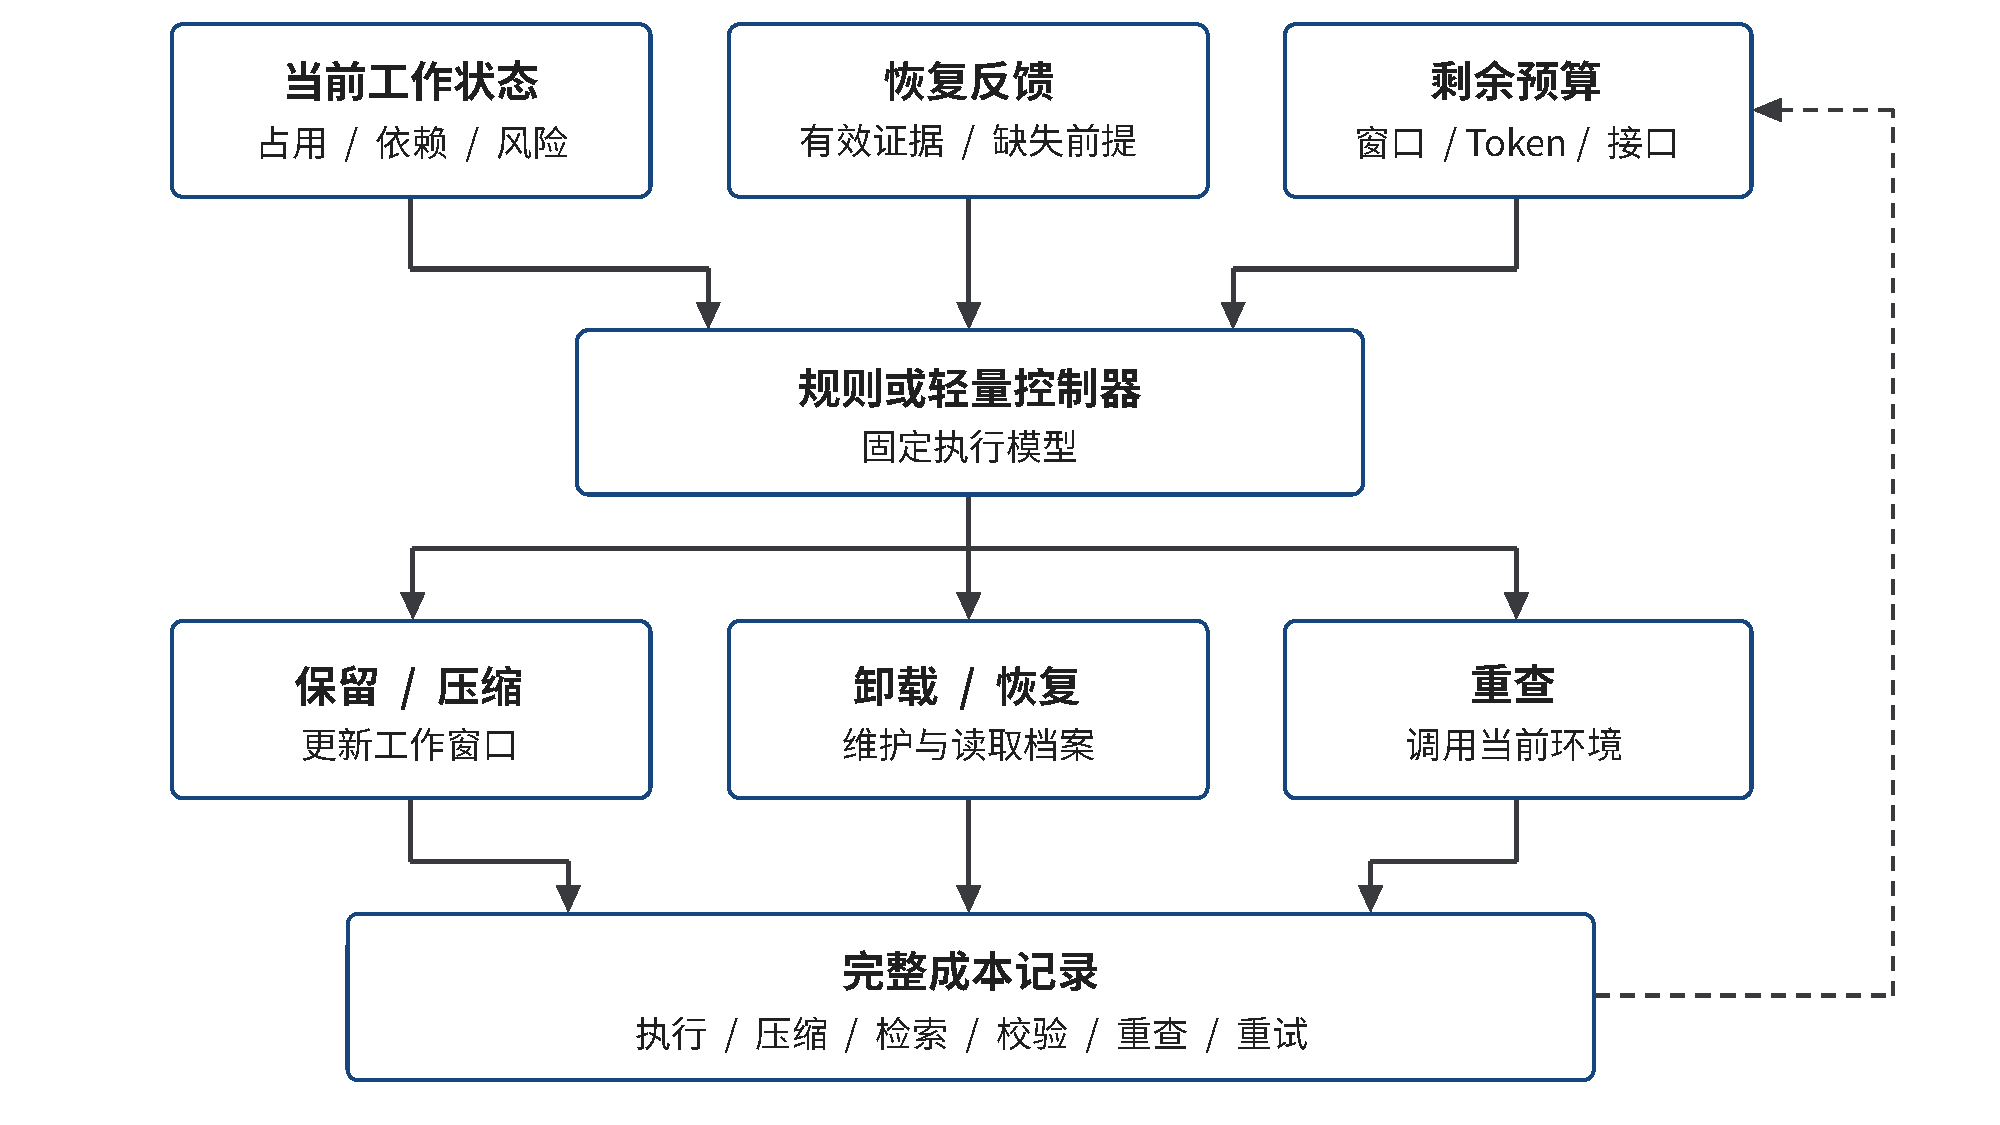
\includegraphics[width=0.98\linewidth]{figures/F05-control.pdf}
\caption{R3结合恢复反馈选择上下文操作并记录全部调用成本}
\label{fig:control}
\end{figure}
% NSFC-ILLUSTRATED END F05


\subsubsection{关键技术}
\textbf{依赖关系的低成本提取与校验。}优先从工具接口约束、对象标识和可验证动作前提出发，辅以模型提取自然语言要求，减少对不可观测内部推理的依赖。关键关系保留原文证据位置，人工核对的是少量争议样本和错误分型；不把所有工具日志转换为复杂知识图谱作为先决条件。对未明确指定的条件不自动补全为确定事实。

\textbf{版本不完备条件下的恢复。}同一对象可能对应多个读取时间与适用范围。恢复机制应先说明当前动作缺少什么，再决定是否需要重查，而非总是取时间最近的片段；有些历史事实本就需要旧版本。缺少可核验时间信息时，系统保留不确定性并限制依赖该事实的动作。实验同时包含“应使用最新状态”和“应追溯历史版本”两类任务，避免把一律选新误当作有效性推理。

\textbf{可解释的错误归因。}每个失败任务按首次可定位错误记录状态遗漏、索引未命中、版本误判、有效证据误用和环境异常，并允许多因共存。环境快照与成对干预用于检验错误归因是否成立；无法定位时标记原因不明，不强行归入某一模块。语言模型评委仅辅助判断自由文本结果，主要行动终态使用程序化测试，并对评委分歧进行人工复核。

\subsubsection{可行性分析}
方法层面，提示压缩、原文回读和可控交互环境均已有可核验实现基础，项目重点在共同条件下组织机制比较及针对性方法改进，无需从零建设通用智能体生态。技术层面，先运行规则和冻结模型，再依据开发证据引入轻量学习，可使失败原因较早暴露。条件层面，现有本地GPU支持中小规模模型和重复实验，昂贵原生训练方法以分层对照或条件性复现安排，不要求完成大规模端到端强化学习。

公开可复位环境能够承担核心证据链。企业数据授权尚未落实时，依然可以通过工具输出膨胀、跨阶段约束与版本变更的受控任务检验方法；这些扰动任务应明确标为构造测试，不称为快手真实业务样本。若依赖—版本交互不成立，项目将保留模块独立效果及全开销边界结论，调整方法复杂度，避免以扩大任务范围掩盖主要假说失败。
